% This is part of Mes notes de mathématique
% Copyright (c) 2011-2013,2016-2017
%   Laurent Claessens
% See the file fdl-1.3.txt for copying conditions.


%+++++++++++++++++++++++++++++++++++++++++++++++++++++++++++++++++++++++++++++++++++++++++++++++++++++++++++++++++++++++++++ 
\section{Isométriques du cube}
%+++++++++++++++++++++++++++++++++++++++++++++++++++++++++++++++++++++++++++++++++++++++++++++++++++++++++++++++++++++++++++
\label{SecPVCmkxM}
\index{isométrie!espace euclidien!isométries du cube}
\index{groupe!et géométrie!isométries du cube}
Les isométries du cube proviennent de \cite{KXjFWKA}.

\begin{wrapfigure}{r}{5.0cm}
   \vspace{-0.5cm}        % à adapter.
   \centering
   \input{auto/pictures_tex/Fig_MCKyvdk.pstricks}
\end{wrapfigure}
Nous considérons le cube centré en l'origine de \( \eR^3\) et \( G\), le groupe des isométries de \( \eR^3\) préservant ce cube. Nous notons aussi \( G^+\) le sous-groupes de \( G\) constitué des éléments de déterminant positif. Nous notons 
\begin{equation}
    \mD=\{ D_1,\ldots, D_4 \}
\end{equation}
l'ensemble des grandes diagonales, c'est à dire les segments \( [AG]\), \( [EC]\), \( [FD]\), et \( [BH]\). Nous savons que \( G\) préserve les longueurs et que ces segments sont les plus longs possibles à l'intérieur du cube. Donc \( G\) agit sur \( \mD\) parce qu'il ne peut transformer une grande diagonale qu'en une autre grande diagonale. Nous avons donc un morphisme de groupes
\begin{equation}
    \rho\colon G\to S_4.
\end{equation}
Nous montrons ce que morphisme est surjectif en montrant qu'il contient les transpositions. Le groupe \( G\) contient la symétrie axiale passant par le milieu \( M\) de \( [AE]\) et le milieu \( N\) de \( CG\). Il est facile de voir que cette symétrie permute \( [AG]\) avec \( [EC]\). De plus elle laisse \( [FD]\) inchangée. En effet, aussi incroyable que cela paraisse en regardant le dessin, nous avons \( FD\perp MN\), parce qu'en termes de vecteurs directeurs,
\begin{equation}
    \begin{aligned}[]
        \vect{ ON }&=\begin{pmatrix}
            1    \\ 
            -1    \\ 
            0    
        \end{pmatrix}&\vect{ OF }&=\begin{pmatrix}
            1    \\ 
            1    \\ 
            -1    
        \end{pmatrix}.
    \end{aligned}
\end{equation}

Étudions à présent le noyau \( \ker(\rho)\). Si \( f\in\ker(\rho)\) n'est pas l'identité, alors \( f(D_i)=D_i\) pour tout \( i\), mais au moins pour une des diagonales les sommets sont inversés. Quitte à renommer les sommets du cube nous supposons que la diagonale \( [AG]\) est retournée : \( f(A)=G\) et \( f(G)=A\). Regardons où peut partir \( B\) sous l'effet de \( f\). Étant donné que \( f\) préserve les diagonales, \( f(B)\in\{ B,C \}\), mais étant donné que \( f\) est une isométrie, \( d\big( f(B),f(G) \big)=d(B,G)\), et nous concluons que \( f(B)=H\). Donc la diagonale \( [BH]\) est retournée sous l'effet de \( f\). En raisonnant de même, nous voyons que \( f\) retourne toutes les diagonales. Donc les éléments non triviaux de \( \ker(\rho)\) retournent toutes les diagonales; il n'y en a donc qu'un seul et c'est la symétrie centrale :
\begin{equation}
    \ker(\rho)=\{ \id,s_0 \}.
\end{equation}
Le premier théorème d'isomorphisme \ref{ThoPremierthoisomo} nous permet d'écrire le quotient de groupes :
\begin{equation}
    \frac{ G }{ \{ \id,s_0 \} }\simeq S_4.
\end{equation}
Une classe d'équivalence modulo \( \ker(\rho)\) dans \( G\) est donc toujours de la forme \( \{ f,f\circ s_0 \}\). Et vu que \( s_0\) est de déterminant \( -1\), une classe contient toujours exactement un élément de déterminant \( 1\) et un de déterminant \( -1\).

D'autre part \( \ker(\rho)\) est normal dans \( G\) parce que en tant que matrice, \( s_0=-\mtu\), donc les problèmes de commutativité ne se posent pas. L'application
\begin{equation}
    \begin{aligned}
        \varphi\colon \frac{ G }{ \{ \id,s_0 \} }&\to G^+ \\
        [g]&\mapsto \begin{cases}
            g    &   \text{si } \det(g)>0\\
            g\circ s_0    &    \text{sinon}
        \end{cases}
    \end{aligned}
\end{equation}
est un isomorphisme de groupes. Et enfin nous pouvons écrire 
\begin{equation}
    G^+\simeq S_4.
\end{equation}

Nous allons maintenant utiliser le corollaire \ref{CoroGohOZ} pour montrer que \( G=G^+\times_{\sigma}\ker(\rho)\). Les conditions sont remplies :
\begin{itemize}
    \item \( \ker(\rho)\) normalise \( G^+\) parce que \( \ker(\rho)\) ne contient que \( \pm\mtu\).
    \item \( \ker(\rho)\cap G^+=\{ \id \}\).
    \item \( \ker(\rho)G^+=G\) parce que les classes d'équivalence de \( G\) modulo \( \ker(\rho)\) sont composées de \( \{ f,f\circ s_0 \}\).
\end{itemize}
Vu que \( G^+\simeq S_4\) et \( \ker(\rho)\simeq \eZ/2\eZ\) nous pouvons écrire de façon plus brillante que
\begin{equation}
    G\simeq S_4\times_{\sigma}\eZ/2\eZ.
\end{equation}
Mais étant donné que la conjugaison par \( s_0\) est triviale, le produit semi-direct est un produit direct :
\begin{equation}
    G\simeq S_4\times\eZ/2\eZ.
\end{equation}
Il est maintenant du meilleur goût de pouvoir identifier géométriquement ces éléments. Les éléments de \( \eZ/2\eZ=\{ \id,s_0 \}\) ne font pas de mystères. Dans \( S_4\) nous avons les classes de conjugaison des éléments \( \id\), \( (12)\), \( (123)\), \( (1234)\) et \( (12)(34)\) déterminées durant l'exemple \ref{ExVYZPzub}.
\begin{enumerate}
    \item
        L'élément \( (12)\) consiste à permuter deux diagonales et laisser les autres en place. Nous avons déjà vu que c'était une symétrie axiale passant par les milieux de deux côtés opposés. Cela fait \( 6\) axes d'ordre \( 2\).
    \item
        L'élément \( (123)\) fixe une des diagonales. C'est donc la symétrie axiale le long de la diagonale fixée. Par exemple la symétrie d'axe \( (AG)\) fait bouger le point \( B\) de la façon suivante :
        \begin{equation}
            B\to D\to E\to B.
        \end{equation}
        C'est une rotation est d'angle \( \frac{ 2\pi }{ 3 }\). Cela sont \( 8\) rotations d'ordre \( 3\).

        Notons à ce propos que la différence entre \( (234)\) et \( (243)\) est que la première fait une rotation d'angle \( 2\pi/3\) tandis que la seconde fait une rotation d'angle \( -2\pi/3\).

    \item
        L'élément \( (1234)\) ne maintient aucune des diagonales et est d'ordre \( 4\). C'est donc la rotation d'angle \( \pi/2\) ou \( -\pi/2\) autour de l'axe passant par les milieux de deux faces opposées. Il y en a \( 6\) comme ça (\( 3\) paires de faces puis pour chaque il y a \( \pi/2\) et \( -\pi/2\)), et ça tombe bien \( 6\) est justement la taille de la classe de conjugaison de \( (1234)\) dans \( S_4\).

    \item
        L'élément \( (12)(34)\) est le carré de la précédente\footnote{En fait c'est \( (13)(24)\), le carré de la précédente, mais c'est la même classe de conjugaison.}, c'est à dire les rotations d'angle \( \pi\) autour des mêmes axes. Cela fait \( 3\) éléments d'ordre \( 2\).
        
\end{enumerate}

%+++++++++++++++++++++++++++++++++++++++++++++++++++++++++++++++++++++++++++++++++++++++++++++++++++++++++++++++++++++++++++ 
\section{Chiffrement RSA}
%+++++++++++++++++++++++++++++++++++++++++++++++++++++++++++++++++++++++++++++++++++++++++++++++++++++++++++++++++++++++++++
\label{SecEVaFYi}
\index{groupe!fini}
\index{groupe!permutation}
\index{groupe!partie génératrice}
\index{anneau!\( \eZ/n\eZ\)}
\index{nombre!premier}

Ce passage sur RSA provient en bonne partie de la \wikipedia{fr}{Rivest_Shamir_Adleman}{la page Wikipédia}.

Alice veut envoyer un message à Bob. L'idée est que Bob va donner à Alice une clef publique qui va permettre de chiffrer le message tandis que Bob va garder pour lui une clef privée qui permet de déchiffrer.

%--------------------------------------------------------------------------------------------------------------------------- 
\subsection{Mise en place par Bob}
%---------------------------------------------------------------------------------------------------------------------------

Bob se crée une paire de clef publique, clef privée de la façon suivante.
\begin{enumerate}
    \item
        Bob choisit deux nombres premiers distincts \( p,q\).
    \item
        Il calcule \( n=pq\) .
    \item
        Par le corollaire \ref{CorlvTmsf}, l'indicatrice d'Euler \( \varphi(n)=(p-1)(q-1)\) est facile à calculer pour Bob.
    \item
        Bob choisit \( e\in \eN\) premier avec \( \varphi(n)\), puis \( d\) tel que \( ed\in[1]_{\varphi(n)}\).
\end{enumerate}
Maintenant la paire est : clef publique \( (n,e)\) et clef privée \( (n,d)\)\footnote{Le fait que \( e\) soit public et \( d\) soit privé est une convention. \( e\) comme  \emph{encryption} et \( d\) comme \emph{decryption}.}.

Bob envoie la paire \( (n,e)\) à Alice. 

\begin{remark}
    Ici nous ne supposons pas que la communication soit sure. Une tierce personne peut intercepter le message. D'ailleurs en principe les gens publient leurs clef publique sur leurs sites, voire sur des sites dédiés. Le problème de l'identification reste à résoudre \wikipedia{en}{Key_signing_party}{à l'ancienne}.
\end{remark}

%--------------------------------------------------------------------------------------------------------------------------- 
\subsection{Chiffrement}
%---------------------------------------------------------------------------------------------------------------------------

Nous chiffrons en utilisant la clef publique \( (n,e)\). D'abord Alice se débrouille pour transformer son message en un nombre plus petit que \( n\). Soit \( M\) ce message. Alice code \( M\) en
\begin{equation}
    C=M^e\mod n.
\end{equation}
Tout le truc est que nous allons voir que l'application \( x\mapsto x^e\) est une bijection de \( \eF_n\) et que l'inverse est facile à calculer par Bob et difficile pour les autres. Alice envoie \( C\) à Bob. Encore une fois, nous ne supposons pas que cette communication soit privée. Le nombre \( C\) peut être intercepté.

%--------------------------------------------------------------------------------------------------------------------------- 
\subsection{Déchiffrement}
%---------------------------------------------------------------------------------------------------------------------------

Nous allons montrer que \( M=C^d\mod n\), et donc que Bob, connaissant \( (n,d)\), peut déchiffrer. D'abord
\begin{equation}
    C^d=(M^e)^d=M^{ed},
\end{equation}
mais nous savons qu'il existe \( k\) tel que
\begin{equation}
    ed=1+k\varphi(n)=1+k(p-1)(q-1).
\end{equation}
L'étape astucieuse est de remarquer que
\begin{equation}    \label{EqreeHgn}
    M^{1+k(p-1)(q-1)}\in [M]_p\cap[M]_q.
\end{equation}
Pour montrer cela nous utilisons le petit théorème de Fermat \ref{ThoOPQOiO} et la remarque \ref{RemCoSnxh}.
\begin{itemize}
    \item Si \( M\) est premier avec \( p\), alors \( M^{p-1}\in[1]_p\).
    \item Si \( M\) n'est pas premier avec \( p\), alors \( M\) est multiple de \( p\) et on sait que \( M^{p-1}\in[0]_p=[M]_p\).
\end{itemize}
Dans les deux cas nous avons \eqref{EqreeHgn}. Le nombre \( M^{1+k\varphi(n)}-M\) est donc à la fois multiple de \( p\) et de \( q\).

Le lemme chinois \ref{LemCtUeGA} nous dit immédiatement\footnote{C'est ici qu'il est important que \( p\) ne soit pas égal à \( q\). Si \( p=q\), alors le lemme chinois ne fonctionne pas.} qu'alors
\begin{equation}
    M^{1+k\varphi(n)}-M
\end{equation}
est un multiple de \( pq=n\), c'est à dire que
\begin{equation}
    C^d=M^{ed}\in [M]_n.
\end{equation}

Si on ne croit pas au lemme chinois, on peut utiliser le lemme de Gauss. Posons
\begin{equation}
    M^{1+k\varphi(n)}-M=ap=bq.
\end{equation}
Dans ce cas \( p\) divise \( bq\), mais \( q\) est premier avec \( p\), donc le lemme de Gauss \ref{LemSdnZNX} nous enseigne\footnote{Ici aussi, si \( p=q\), ça ne marche pas.} que \( p\) divise \( b\).

%--------------------------------------------------------------------------------------------------------------------------- 
\subsection{Une imprudence à ne pas commettre}
%---------------------------------------------------------------------------------------------------------------------------

Nous avons pris deux cas selon que \( M\) soit ou non premier avec \( p\). Une question qui se pose est la suivante : est-ce que c'est une bonne idée d'envoyer un message qui ne soit pas premier avec \( p\) ?

Si nous savons que \( M\) n'est pas premier avec \( p\), alors nous avons \( M^e=l^ep^e\) et \( n=pq\) qui sont publics. Donc un calcul de PGCD permettrait de trouver \( p\).

Il faut cependant savoir que \label{PageAKTBooMDeQxY}
\begin{itemize}
    \item La probabilité que ça arrive est infime : vu que \( M\) est entre \( 0\) et \( n=pq\), les multiples de \( p\) possibles sont \( p,2p,\cdots pq\). Il y a dont une chance sur \( p\) que cela arrive. Typiquement avec des si \( p\) de l'ordre de \( 10^{120}\), on peut utiliser RSA chaque milliseconde sur chaque atome de l'univers depuis le début des temps que ça ne se serait presque certainement pas encore produit.
    \item
        De toutes façons Alice ne sait pas vérifier si son message est premier avec \( p\) parce qu'elle ne connaît pas \( p\).
    \item 
        En conclusion la partie de la preuve qui montre que \( M^{1+\varphi(n)}\in [M]_p\cap[M]_q\) dans le cas \( M\) non premier avec \( p\) est, à toutes fins pratiques, inutile parce que ce cas de figure ne se présentera jamais dans toutes l'histoire de l'univers, même pas avec une civilisation intelligente autour de chaque étoile.
\end{itemize}

\begin{probleme}\label{ProbGAYFooZATuYy}
    Est-ce que ces trois points sont corrects ?
\end{probleme}

%--------------------------------------------------------------------------------------------------------------------------- 
\subsection{Problèmes calculatoires}
%---------------------------------------------------------------------------------------------------------------------------

Pour implémenter RSA, il faut pouvoir faire (au moins) trois choses :
\begin{enumerate}
    \item
        Trouver de grands nombres premiers.
    \item
        Trouver des couples de Bézout.
    \item
        Calculer \( M^e\) lorsque \( e\) est très grand.
\end{enumerate}
En ce qui concerne le problème de trouver des nombres premiers, c'est compliqué, mais il faut savoir qu'il y en a plein. À \( 120\) chiffres, il y a environ autant de nombres premiers que d'atomes dans \( 10^{20}\) fois l'univers connu. Cela rend impossible toute tentative de factoriser un grand nombre en essayant toutes les possibilités. Même pas en science-fiction\footnote{Cela donne une idée des connaissances en math des klingons, dont le docteur Spock parvient à craquer le code mentalement en deux heures.}.

Trouver des nombres \( u\) et \( v\) tels que \( Au+Bv=\pgcd(A,B)\) est un problème expliqué en \ref{subSecIpmnhO}.

En ce qui concerne le calcul de \( M^e\) lorsque \( e\) est grand, il n'est évidemment pas pensable de faire \( M\cdot M\cdot\ldots M\) avec \( e\) facteurs. Un truc pour calculer en moins d'étapes est l'\defe{exponentiation rapide}{exponentielle!rapide}. Si \( e=2k\) est pair, nous calculons
\begin{equation}
    M^e=(M^k)^2;
\end{equation}
si \( e=2k+1\) alors nous calculons
\begin{equation}
    M^e=M(M^k)^2.
\end{equation}
Le calcul prend alors seulement environ \(  \log_2(e)  \) étapes. Pour donner une idée,
\begin{equation}
    \log_2(10^{120})\simeq 400.
\end{equation}
Très raisonnable, mais un ordinateur reste indispensable.

%--------------------------------------------------------------------------------------------------------------------------- 
\subsection{La solidité de RSA}
%---------------------------------------------------------------------------------------------------------------------------

La solidité de la méthode repose sur deux conjectures (non démontrées !!) :
\begin{itemize}
    \item Pour déchiffrer il \emph{faut} connaitre \( p\) et \( q\). 
    \item La difficulté de trouver \( p\) et \( q\) en partant de \( n=pq\) est exponentielle en \( n\).
\end{itemize}
Dans la méthode de déchiffrage proposée ici, \( p\) et \( q\) sont utilisés pour calculer \( d\) qui est solution de \( ed=[1]_{\varphi(n)}\). La seule formule connue pour calculer \( \varphi(n)\) est \( \varphi(n)=(p-1)(q-1)\). Si on trouve plus simple, alors RSA peut être craqué.

%--------------------------------------------------------------------------------------------------------------------------- 
\subsection{Note non mathématique pour doucher l'enthousiasme}
%---------------------------------------------------------------------------------------------------------------------------

Il est souvent dit\cite{ooTODUooAhFHQk} que différents systèmes de chiffrement peuvent aider à avoir des discussions «discrètes» dans les régimes totalitaires. La technologie au service de la démocratie, voila qui enthousiasme la jeunesse\footnote{Cela dit, le navigateur Tor\cite{ooHBLCooYtBBfx}, qui est un pur produit de RSA, permet effectivement d'accéder en France aux sites bloqués pour apologie du terrorisme (mars 2015).}. La réalité est qu'il est souvent possible de craquer un système de chiffrement arbitrairement complexe, même sans connaitre le petit théorème de Fermat \ldots

\notbool{isBook}{
\begin{center}
            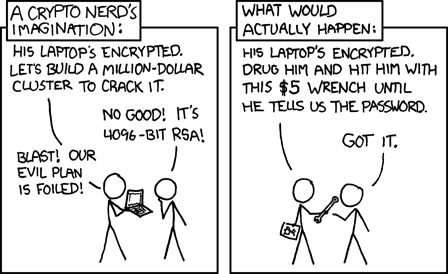
\includegraphics[width=10cm]{pictures_bitmap/security.png}\\
        \url{http://xkcd.com/538/} \href{http://creativecommons.org/licenses/by-nc/2.5/}{ Creative Commons Attribution-NonCommercial 2.5 License}.
\end{center}%
}{}            

\noindent \ldots tout dépends du contexte.

